\section{Durchführung}

\subsection{Aufbau}
In diesem Versuch wird die Lebensdauer kosmischer Myonen mithilfe dem in Abb. \ref{fig:Aufbau} gezeigten Aufbau bestimmt. Ein Foto des Aufbaus ist in Abb. \ref{fig:Aufbau_Foto} zu sehen. Die einzelnen Bauteile werden im Folgenden kurz beschrieben.
\begin{itemize}
    \item Szintillator:
    \item Photomultiplier
    \item Verzögerungsleitung 
    \item Diskriminator
    \item Koinzidenzschaltung
    \item AND-Gatter
    \item Monostabile Kippstufe (Univibrator)
    \item Zeit-Amplituden-Converter (TAC)
    \item Vielkanalanalysator
\end{itemize}

\begin{figure}
    \centering
    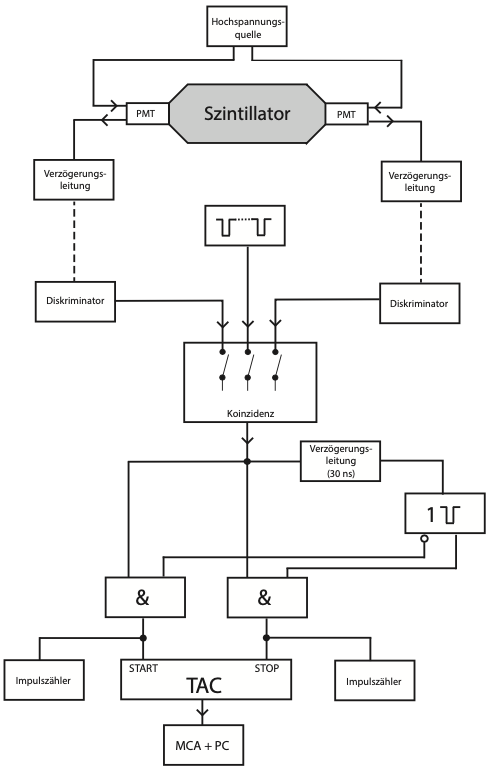
\includegraphics[width=0.7\linewidth]{figures/Aufbau.png}
    \caption{Blockschaltbild der Versuchsvorrichtung. \cite{V01}}
    \label{fig:Aufbau}
\end{figure}

\begin{figure}
    \centering
    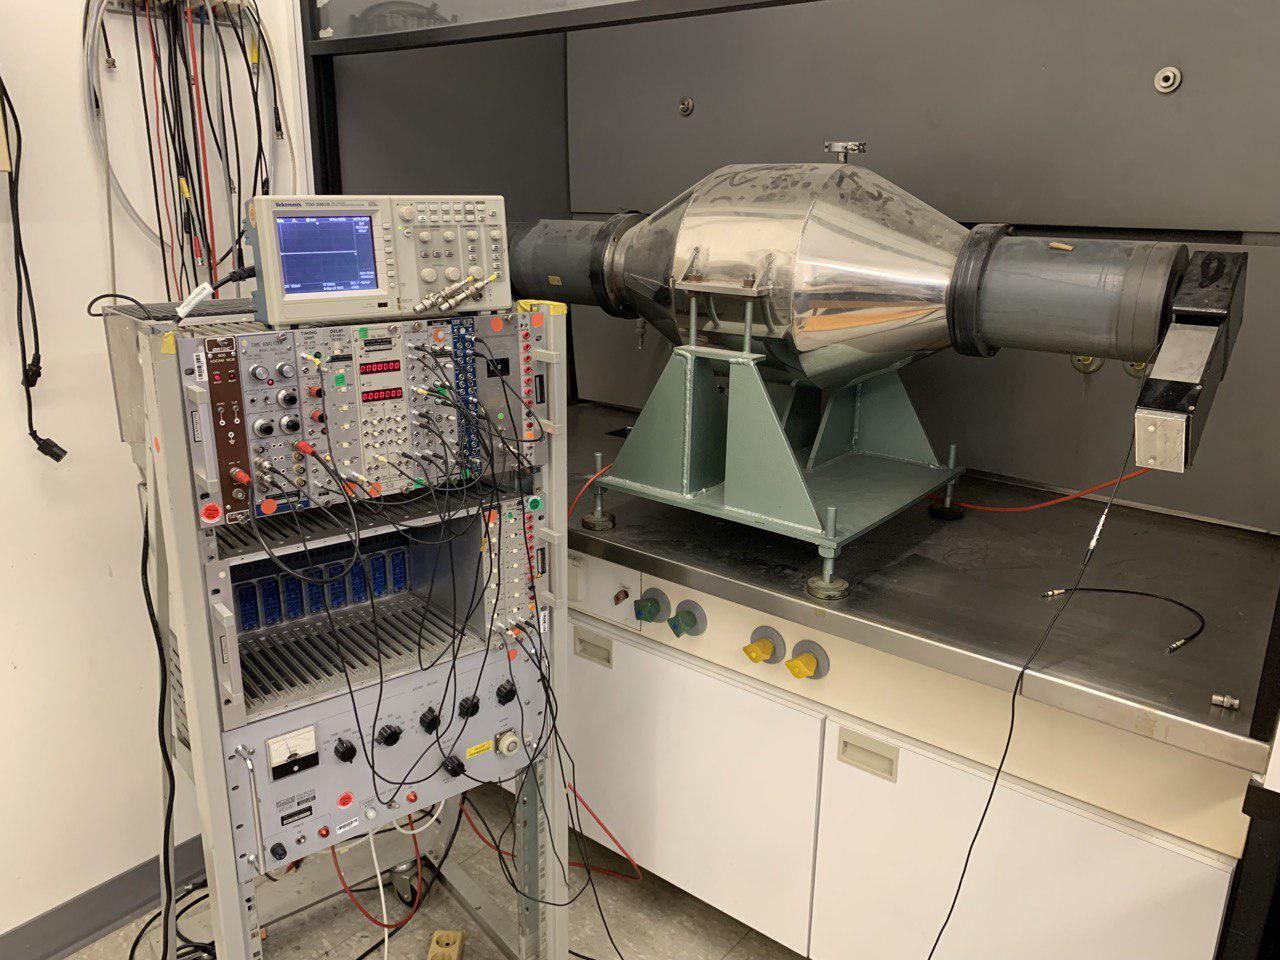
\includegraphics[width=0.7\linewidth]{figures/Aufbau_Foto.jpg}
    \caption{Foto des Versuchsaufbaus.}
    \label{fig:Aufbau_Foto}
\end{figure}

\subsection{Kalibrierung und Verkabelung}
Zunächst werden die am Szintillationstank angebrachten Photomultiplier an ein Oszilloskop angeschlossen, um sicherzustellen, dass sie funktionieren.
Anschließend werden die Photomultiplier über die Verzögerungsleitungen mit den Diskriminatoren verkabelt. Es wird noch keine Verzögerung eingestellt. Das Ergebnis wird ebenfalls am Oszilloskop sichtbar gemacht. An den Diskriminatoren wird die Pulsweite mithilfe der am Oszilloskop abgebildeten Pulse auf jeweils $\Delta t = \SI{10}{\nano\second}$ gestellt.
Als nächstes werden die Ausgänge der Diskriminatoren an einen Impulszähler angeschlossen. Die Schwelle der Diskriminatoren wird so angepasst, dass an beiden Ausgängen ca. $\num{30}$ Pulse pro Sekunde gemessen werden.
Im nächsten Schritt wird die Koinzidenz in die Schaltung integriert und der Ausgang an den Impulszähler angeschlossen. Die Verzögerungen werden systematisch nacheinander variiert. Dabei wird für jede Verzögerung die Impulsrate aufgenommen. Es ist ein deutliches Maximum, bzw. ein Plateau in der Verteilung, der Impulsrate zu sehen. Die Verzögerung wird auf diesen Wert eingestellt.
Die restliche Schaltung wird verkabelt. 
Am Monoflop wird eine Suchzeit $T_s$ eingestellt, die am auch TAC entsprechend eingestellt wird.

Der Teil vor der Koinzidenzschaltung wird abgeklemmt. Stattdessen wird ein Doppelimpulsgenerator an die Koinzidenz angeschlossen.
Die Pulsabstände werden zwischen $\SI{0.3}{\micro\second}$ und $\SI{9.9}{\micro\second}$ variiert und die entsprechende Kanalnummer des Vielkanalanalysators aufgenommen.

\subsection{Messung}
An die Koinzidenzschaltung werden erneut die zuvor abgeklemmten Photomultiplier angeschlossen. Die Aufzeichung des Vielkanalanalysators wird gleichzeitig mit dem Impulszähler gestartet und etwa $\num{20}$ bis $\SI{30}{\hour}$ laufen gelassen. %wie lange genau? Weiß man das? 